%!TEX program = lualatex
\documentclass[12pt,letterpaper,twoside]{article}
%!TEX root = ./set_cover_problem.tex

% Pro­gram­ming fa­cil­i­ties
	\usepackage{etoolbox}
	\usepackage{ifxetex}
	\usepackage{ifluatex}

% Encoding
	\usepackage[T1]{fontenc}
	\ifboolexpr{bool{xetex} or bool{luatex}}{%
		\usepackage{fontspec}
	}{%
		\usepackage[utf8]{inputenc}
	}

% Language
	\usepackage[english,french]{babel} % Second language = main language

% Show a summary of the layout of the current document with \layout.
	%\usepackage{layout}

% For easy management of document margins and the document page size.
	\usepackage[top=2cm, bottom=1.8cm, left=1.8cm, right=1.8cm, head=14pt, foot=36pt]{geometry}

% Lets you change line spacing.
	%\usepackage{setspace}

% Euro symbol
	%\usepackage{eurosym}

% Fonts (include only one)
	%\usepackage{bookman}
	%\usepackage{charter}
	%\usepackage{newcent}
	\usepackage{lmodern}
	%\usepackage{mathpazo}
	%\usepackage{mathptmx}

% Enables typesetting of hyperlinks
	%\usepackage{url}
	\usepackage{hyperref}

% Verbatim environment
	%\usepackage{verbatim}
	%\usepackage{moreverb}
	\usepackage{fancyvrb}

% Code listing
	\usepackage{listings}

% To change header and footer of any page of the document.
	\usepackage{fancyhdr}

% Allows you to insert graphic files within a document.
	%\usepackage{graphicx}

% Allows figures or tables to have text wrapped around them.
	%\usepackage{wrapfig}

% Adds support for colored text.
	\usepackage{xcolor}

% Allows tables rows and columns to be colored, and even individual cells.
	%\usepackage{colortbl}

% Mathematics
	\usepackage{amsmath}
	\usepackage{amssymb}
	\usepackage{mathrsfs}
	\usepackage{amsthm}
	\usepackage{dsfont}
	\usepackage{braket}
	\usepackage{stmaryrd}
	%\usepackage{mathtools}
	%\usepackage{bm} % Greek letters in math mode

% Tables
	\usepackage{array}
	\usepackage{tabularx}
	\usepackage{multirow}
	\usepackage{booktabs}

% Provides control over the layout of the three basic list environments: enumerate, itemize and description.
	%\usepackage{enumitem}

% Interface to sectioning commands for selection from various title styles
	\usepackage[nobottomtitles]{titlesec}

% Highly customized stacking of objects, insets, baseline changes, etc.
	\usepackage{stackengine}

% Routines for constrained scaling and stretching of objects, relative to a reference object or in absolute terms
	\usepackage{scalerel}

% \rel­size command
	\usepackage{relsize}

% Provides control over the typography of the Table of Contents, List of Figures and List of Tables, and the ability to create new ‘List of ...’.
	\usepackage{tocloft}
	\usepackage{titletoc}

% Advanced bibliography handling.
	%\usepackage{bibtex}
	\usepackage[backend=bibtex,bibstyle=ieee,citestyle=numeric-comp]{biblatex}

% Allows customization of appearance and placement of captions for figures, tables, etc.
	\usepackage[justification=centering]{caption}

% Provides the multicols environment which typesets text into multiple columns.
	%\usepackage{multicol}

% This package simplifies the insertion of external multi-page PDF or PS documents.
	%\usepackage{pdfpages}

% Prints out all index entries in the left margin of the text.
	%\usepackage{showidx}

% Allow to define multiple floats (figures, tables) within one environment giving individual captions and labels in the form 1a, 1b.
	%\usepackage{subcaption}

% Allow TeX pictures or other TeX code to be compiled standalone or as part of a main document
	%\usepackage[subpreambles=true]{standalone}
	\usepackage[mode=tex]{standalone}
	\usepackage{import}

% Floating elements placement
	\usepackage{float}

% PGF-TikZ
	\usepackage{pgf}
	\usepackage{pgfplots}
	\pgfplotsset{compat=1.16}
	\usepackage{tikz}
	\usepackage{tikzpeople}

% Lets you insert notes of stuff to do with the syntax \todo{Add details.}.
	%\usepackage{todonotes}

% Text Companion fonts, which provide many text symbols (such as baht, bullet, copyright, musicalnote, onequarter, section, and yen), in the TS1 encoding.
	\usepackage{textcomp}

% Add document elements like a bibliography or an index to the Table of Contents.
	\usepackage[notindex,nottoc,notlot,notlof]{tocbibind}

%!TEX root = ./PARL.tex

%=======================================================================================================
%=============================================== Informations ==========================================
%=======================================================================================================

% Cover infos
\title{Rapport intermédiaire: problème de couverture d'ensemble}
\author{Benoît Cortier \& Maxime Pinard}
\date{\today{}}

% Fancy style options
\lhead{\small Benoît Cortier \& Maxime Pinard}
\rhead{\small Couverture d'ensemble}
\chead{}
\lfoot{}
\rfoot{}
\cfoot{\thepage}
\pagestyle{fancy}

%% Redefine the fancy plain page style
%\fancypagestyle{plain}{
%	\fancyhf{}
%	\lhead{\small Benoît Cortier \& Maxime Pinard}
%	\rhead{\small PARL}
%	\chead{}
%	\lfoot{}
%	\rfoot{}
%	\cfoot{\thepage}
%}

%=======================================================================================================
%================================================== Configs ============================================
%=======================================================================================================

% Figures folder
\graphicspath{{figures/}}

% Prevent page breaks in paragraphs
\predisplaypenalty=1000
\postdisplaypenalty=1000
\clubpenalty=1000

% Minimal space required in the bottom margin not to move the title on the next page
\renewcommand{\bottomtitlespace}{.1\textheight}

% Links config, especialy for the table of contents
\hypersetup{
    colorlinks=true,
    linkcolor=black,
    urlcolor=blue,
    linktoc=all
}

% French language config
\frenchbsetup{StandardLayout=true,ReduceListSpacing=false,CompactItemize=false}

% Environments
\theoremstyle{definition}
\newtheorem{thm}{Théorème}
\newtheorem{defn}{Définition}
\newtheorem{prop}{Proposition}

%=======================================================================================================
%================================================= Functions ===========================================
%=======================================================================================================

% Clear to the next left page
\newcommand*{\cleartoleftpage}{
  \clearpage \ifodd\value{page}\hbox{}\newpage\fi
}

% Paragraph with line break
\newcommand{\p}[1]{\paragraph{#1\\}}

% Function to print a warning sign
\newcommand{\dangersign}[1][2.5ex]
	{\renewcommand{\stacktype}{L}
		{\scaleto{\stackon[1pt]{\color{red}$\triangle$}{\fontsize{4pt}{4pt}\selectfont !}}{#1}}}

% Definition of some dt/dx/dy shortcuts for integrals
\newcommand{\dt}
{\;\mathrm{d}\,t}

\newcommand{\dx}
{\;\mathrm{d}\,x}

\newcommand{\dy}
{\;\mathrm{d}\,y}

% Definition of \Witem for 'itemize' environment with a warning sign
\newcommand{\Witem}
{\item[\dangersign{}]}

% Definition of a Max function shortcut
\newcommand{\Max}[2][ ]
{\underset{#1}{\text{Max}}\,#2}


\bibliography{references}
\nocite{*}

\begin{document}
	\maketitle{}
	\tableofcontents{}
	\newpage{}
	\section{Définition du problème}
		\subsection{SCP et WSCP}
			\paragraph*{Présentation\\}
				Le problème de couverture d'ensemble, ou \emph{Set Covering Problem} (SCP),
				fait parti des 21 problèmes NP-complets de \citeauthor{Karp1972}~\cite{Karp1972}
				et est NP-complet au sens fort \cite{garey2002computers}.
			\paragraph*{Problème de couverture d'ensemble\\}
				Étant donné un ensemble univers \(U = \{u_1, u_2, u_3, \dots, u_n\}\) et une famille \(S = \{s_1, s_2, \dots, s_m\}\) de sous-ensembles de \(U\),
				le problème consiste à trouver une sous-famille de \(S\) la plus petite possible permettant de couvrir chaque élément de \(U\)
				au moins une fois. Un élément \(e\) de \(U\) est couvert par un sous-ensemble \(A\) si \(e \in A\).
			\paragraph*{Problème de couverture d'ensemble pondéré\\}
				En associant un coût positif \(c_i\) à chaque sous-ensemble, on obtient le problème de couverture d'ensemble pondéré ou \emph{Weighted Set Covering Problem} (WSCP) et	l'objectif est alors de déterminer une couverture de coût minimum.~\cite{Vazirani2003}
		\subsection{Utilité}
			\paragraph*{}
				Une grande variété de problèmes de positionnement, de distribution, de planification et autres peuvent être formulés comme variantes du problème de couverture d'ensemble. Parmi les problèmes réels auxquels cette approche a été appliquée avec succès:\cite{Balas1982}
				\begin{itemize}
					\item problèmes de sélection de sites et d'allocation d'emplacement
					\item emplacement des installations des services d'urgence (casernes de pompiers, hôpitaux, etc.)
					\item choix de la taille et de l'emplacement des plates-formes de forage dans les champs pétrolifères en mer
					\item horaire des équipages pour les compagnies aériennes, les compagnies de bus, les chemins de fer
					\item répartition des fréquences de radiodiffusion entre stations de radio ou de télévision
					\item recherche d'informations (à partir de fichiers informatiques)
					\item \ldots
				\end{itemize}
	\section{Exemple minimal}
		\subsection{SCP}
			\paragraph*{}
				Soit un ensemble univers \(U = \{u_1, u_2, \dots, u_{12}\}\) (représenté par des points sur le figure \ref{fig:example}) et une famille \(S = \{s_1, s_2, \dots, s_6\}\) de sous-ensembles de \(U\) (représentés par des rectangles sur la figure \ref{fig:example}) avec:
				\begin{itemize}
					\item \(s_1 = \{u_1, u_2, u_3, u_4, u_5, u_6\}\)
					\item \(s_2 = \{u_5, u_6, u_8, u_9\}\)
					\item \(s_3 = \{u_1, u_4, u_7, u_{10}\}\)
					\item \(s_4 = \{u_2, u_5, u_8, u_{11}\}\)
					\item \(s_5 = \{u_3, u_6, u_9, u_{12}\}\)
					\item \(s_6 = \{u_{10}, u_{11}, u_{12}\}\)
				\end{itemize}
			\paragraph*{}
				La solution optimale à cette instance est la sous famille \(S'=\{s_3, s_4, s_5\}\) (colorée en gris sur la figure \ref{fig:example}).
			\begin{figure}[H]
				\centering%
				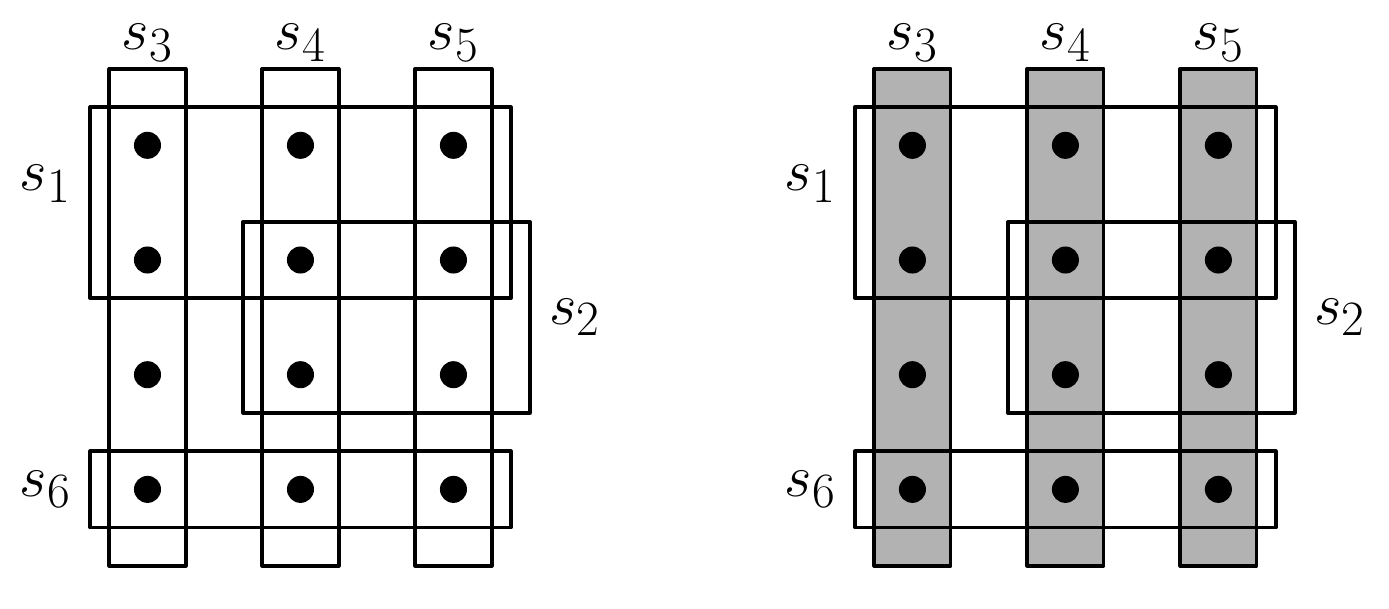
\includegraphics[width=0.65\linewidth]{figures/example}%
				\caption{Exemple d'instance du Set Cover Problem et solution optimale\cite{Mount2017}}%
				\label{fig:example}%
			\end{figure}
		\subsection{WSCP}
			TODO
	\section{Complexité}
		\paragraph*{}
			Le SCP est un problème d'optimisation NP-difficile, et NP-complet dans sa forme décisionnelle. IL fait notamment parti des 21 problèmes NP-complets de \citeauthor{Karp1972}~\cite{Karp1972} et est NP-complet au sens fort \cite{garey2002computers}.
		\paragraph*{}
			La démonstration de la NP-complétude du problème a été réalisée par \citeauthor{Karp1972} en \citeyear{Karp1972} dans son article \citetitle{Karp1972}\cite{Karp1972}. Dans cet article, il réalise des réductions pour 21 problèmes réputés difficiles de combinatoire et de théorie des graphes comme représenté sur la figure \ref{fig:karp_reduction_tree}.
		\begin{figure}[H]
			\centering%
			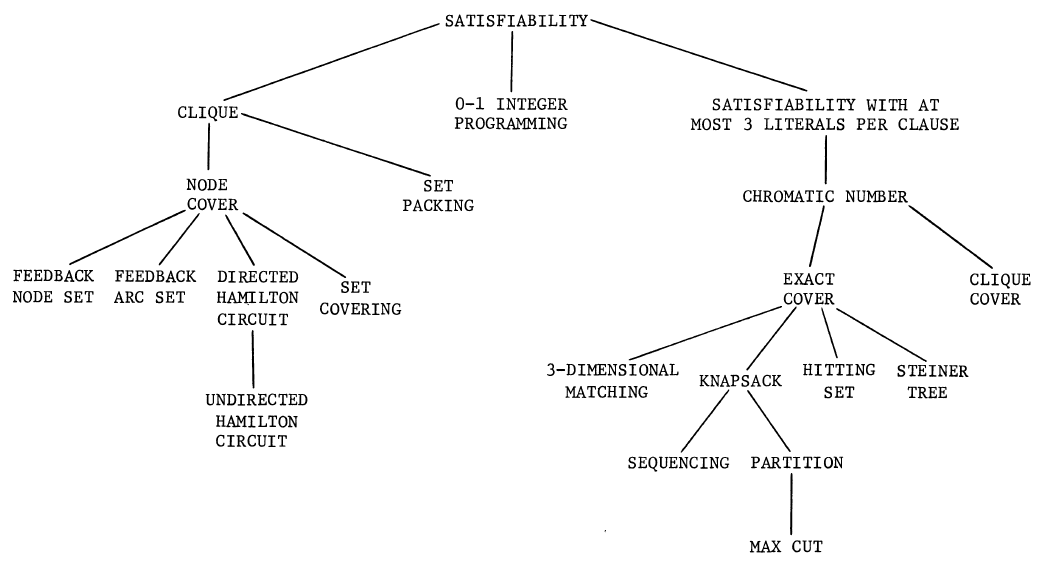
\includegraphics[width=\linewidth]{karp_reduction_tree}%
			\caption{Arbre des réductions réalisées par Karp\cite{Karp1972}}%
			\label{fig:karp_reduction_tree}%
		\end{figure}
		\paragraph*{}
			Concernant notre problème, \citeauthor{Karp1972} montre donc que le Boolean Satisfiability Problem (SATISFIABILITY) peut être réduit au Clique Problem (CLIQUE) qui peut etre réduit au Vertex/Node Cover Problem (NODE COVER) qui peut être réduit au Set Covering Problem (SET COVERING).
		\paragraph*{}
			Le théorème de Cook–Levin et sa démonstration publié en \citeyear{Cook1971} par \citeauthor{Cook1971} dans l'article \citetitle{Cook1971}\cite{Cook1971} prouve le Boolean Satisfiability Problem comme étant un problème NP-complet. Par réduction, le Set Covering Problem est donc aussi NP-complet.
		\paragraph*{}
			Pour ce qui est du Weighted Set Covering Problem (WSCP), c'est une généralisation du SCP et la réduction de ce dernier est évidente, il suffit de rajouter des poids tous égaux a une instance de SCP pour obtenir une instance de WSCP équivalente, le WSCP est donc lui aussi NP-complet.
	\section{Représentations}
		\subsection*{Représentation du problème}
			matrice \(a_{i,j} (n \times m)\)
		\subsection{Représentation des solutions}
			bitset

	\section{Instances du problème}
		\paragraph*{}
			On utilise les groupes d'instances mis a disposition par \citeauthor{OR-Library} dans son regroupement d'instances OR-Library\cite{OR-Library}. Parmis ces instances, celles de 4 à 6 proviennent l'article \citetitle{Balas1980}\cite{Balas1980} de \citeauthor{Balas1980}, celles de A à D proviennent de l'article \citetitle{Beasley1987}\cite{Beasley1987} de \citeauthor{Beasley1987} et celles de E à H proviennent de l'article \citetitle{Beasley1990}\cite{Beasley1990} de \citeauthor{Beasley1990}.
		\paragraph*{}
			Toutes les instances du problème de ces groupes on été générées en utilisant le shémas de \citeauthor{Balas1980}\cite{Balas1980} dans lequel le cout \(c_i\) de chaque colonne \(i\) est pris aléatoirement dans l'intervalle \(\llbracket0,100\rrbracket\), chaque colonne couvre au moins une ligne et chaque ligne est couverte par au moins deux clonnes.
		\paragraph*{}
		   Les propriétés de ces groupes d'instances sont décrites dans la table \ref{table:scp_problem_sets}, la densitée étant la proportion de \(1\) dans la matrice \(a_{i,j}\). La table \ref{table:problem_optimal_solutions}, contient les valeure optimales pour les problèmes pour lesquels elle est connue.
		\begin{table}[H]
			\centering
			%!TEX root = ../set_cover_problem.tex
\begin{tabular}{*{5}{C{65pt}}}
	\toprule
	Groupe d'instances & Nombre de lignes (\(m\)) [points] & Nombre de colonnes (\(n\)) [sous-ensembles] & densité (\%) & Nombre d'instances du groupe\\
	\midrule
	4 & 200 & 1000 & 2 & 10\\
	5 & 200 & 2000 & 2 & 10\\
	6 & 200 & 1000 & 5 & 5\\
	A & 300 & 3000 & 2 & 5\\
	B & 300 & 3000 & 5 & 5\\
	C & 400 & 4000 & 2 & 5\\
	D & 400 & 4000 & 5 & 5\\
	E & 500 & 5000 & 10 & 5\\
	F & 500 & 5000 & 20 & 5\\
	G & 1000 & 10000 & 2 & 5\\
	H & 1000 & 10000 & 5 & 5\\
	\bottomrule
\end{tabular}
			\caption{Groupes d'instances du SCP utilisées\cite{OR-Library,Balas1980,Beasley1987,Beasley1990}}
			\label{table:scp_problem_sets}
		\end{table}
		\begin{table}[H]
			\centering
			\begin{minipage}[t]{0.45\linewidth}
				\centering
				%!TEX root = ../set_cover_problem.tex
\begin{tabular}{*{2}{C{65pt}}}
	\toprule
	Problem number & Optimal solution value\\
	\midrule
	4.1 & 429\\
	4.2 & 512\\
	4.3 & 516\\
	4.4 & 494\\
	4.5 & 512\\
	4.6 & 560\\
	4.7 & 430\\
	4.8 & 792\\
	4.9 & 641\\
	4.10 & 514\\
	\midrule
	5.1 & 253\\
	5.2 & 302\\
	5.3 & 226\\
	5.4 & 242\\
	5.5 & 211\\
	5.6 & 213\\
	5.7 & 293\\
	5.8 & 288\\
	5.9 & 279\\
	5.10 & 265\\
	\bottomrule
\end{tabular}
			\end{minipage}
			\begin{minipage}[t]{0.45\linewidth}
				\centering
				%!TEX root = ../set_cover_problem.tex
\begin{tabular}{*{2}{C{65pt}}}
	\toprule
	Problem number & Optimal solution value\\
	\midrule
	A.1 & 253\\
	A.2 & 252\\
	A.3 & 232\\
	A.4 & 234\\
	A.5 & 236\\
	\midrule
	B.1 & 69\\
	B.2 & 76\\
	B.3 & 80\\
	B.4 & 79\\
	B.5 & 72\\
	\midrule
	C.1 & 227\\
	C.2 & 219\\
	C.3 & 243\\
	C.4 & 219\\
	C.5 & 215\\
	\midrule
	D.1 & 60\\
	D.2 & 66\\
	D.3 & 72\\
	D.4 & 62\\
	D.5 & 61\\
	\bottomrule
\end{tabular}
			\end{minipage}
			\caption{Solutions optimales des instances du SCP utilisée\cite{Beasley1990}}
			\label{table:problem_optimal_solutions}
		\end{table}
	\section{Méthode exacte}
		\paragraph*{}
			Il existe une méthode exacte plus efficace qui utilise la méthode Branch and Bound ainsi que le Simplexe (pour résoudre une version
			du problème linéaire relaxée)~\cite{caprara2000algorithms}.
	\section{Méthodes approchées}
		TODO
	\newpage\printbibliography[heading=bibintoc]{}
\end{document}

% Problem set        Files
% 4                  scp41, ..., scp410
% 5                  scp51, ..., scp510
% 6                  scp61, ..., scp65
% A                  scpa1, ..., scpa5
% B                  scpb1, ..., scpb5
% C                  scpc1, ..., scpc5
% D                  scpd1, ..., scpd5
% E                  scpe1, ..., scpe5

% Problem set        Files
% E                  scpnre1, ..., scpnre5
% F                  scpnrf1, ..., scpnrf5
% G                  scpnrg1, ..., scpnrg5
% H                  scpnrh1, ..., scpnrh5
